\documentclass[11pt,a4paper]{article}
\usepackage[utf8]{vietnam}
\usepackage{amsmath,amssymb}
\usepackage{tabularx}
\usepackage{tikz}
\usepackage{xcolor}
\usepackage{fancyhdr}
\usepackage[top=1.8cm, bottom=2.0cm, left=1.8cm, right=1.8cm]{geometry}

\setlength{\parskip}{3pt}
\setlength{\parindent}{0pt}

\pagestyle{fancy}
\fancyhf{}
\renewcommand{\headrulewidth}{0.4pt}
\lhead{\footnotesize \textbf{CHÙA HƯƠNG SƠN -- ÔN THI VÀO 10}}
\rhead{\footnotesize \textbf{ĐỀ THI THỬ CUỐI HỌC KỲ I (ĐỀ SỐ 09)}}
\cfoot{\thepage}

\begin{document}

\noindent
\begin{tabular*}{\linewidth}{@{\extracolsep{\fill}}cc@{}}
\textbf{SỞ GIÁO DỤC VÀ ĐÀO TẠO} & \textbf{ĐỀ KIỂM TRA CUỐI HỌC KỲ I} \\
\textbf{CHÙA HƯƠNG SƠN} & \textbf{NĂM HỌC 2026 -- 2027} \\
\textbf{ĐỀ THI THỬ SỐ 09} & \textbf{MÔN: TOÁN -- LỚP 9} \\
\textit{(Đề thi gồm 03 trang)} & \textit{Thời gian làm bài: 90 phút (không kể thời gian phát đề)} \\
\end{tabular*}

\vspace{2mm}
\noindent
\rule{\linewidth}{0.8pt}

\vspace{1mm}
\noindent
Họ và tên thí sinh: \dotfill Số báo danh: \dotfill

\vspace{2mm}
\noindent
\textbf{\large I. TRẮC NGHIỆM KHÁCH QUAN (7,0 điểm)}

\vspace{1mm}
\noindent
\textbf{Phần 1. Trắc nghiệm nhiều lựa chọn (3,0 điểm).} \textit{Từ câu 1 đến câu 12, thí sinh chọn đáp án đúng nhất trong 4 đáp án A, B, C, D rồi ghi vào bài làm.}

\vspace{1.5mm}
\textbf{Câu 1.} Giá trị của biểu thức $2\sqrt{50} - 3\sqrt{18} + \sqrt{32}$ bằng\\
\begin{tabularx}{\linewidth}{XXXX}
\textbf{A.} $5\sqrt{2}$. & \textbf{B.} $6\sqrt{2}$. & \textbf{C.} $4\sqrt{2}$. & \textbf{D.} $3\sqrt{2}$.
\end{tabularx}

\vspace{1.5mm}
\textbf{Câu 2.} Trong các khẳng định sau về tỉ số lượng giác của góc nhọn, khẳng định nào đúng?\\
\begin{tabularx}{\linewidth}{XXXX}
\textbf{A.} $\cos 60^\circ = \dfrac{1}{2}$. & \textbf{B.} $\sin 60^\circ = \dfrac{1}{2}$. & \textbf{C.} $\tan 45^\circ = \dfrac{\sqrt{2}}{2}$. & \textbf{D.} $\cot 30^\circ = \dfrac{\sqrt{3}}{3}$.
\end{tabularx}

\vspace{1.5mm}
\textbf{Câu 3.} Bất phương trình nào dưới đây là bất phương trình bậc nhất một ẩn?\\
\begin{tabularx}{\linewidth}{XXXX}
\textbf{A.} $7x + 21 > 0$. & \textbf{B.} $0x - 9 \le 0$. & \textbf{C.} $x^2 + 5x \ge 0$. & \textbf{D.} $\dfrac{2}{x+1} < 0$.
\end{tabularx}

\vspace{1.5mm}
\textbf{Câu 4.} Cho hai số thực $m$ và $n$ thỏa mãn $m > n$. Khẳng định nào sau đây là luôn đúng?\\
\begin{tabularx}{\linewidth}{XXXX}
\textbf{A.} $m - 3 > n - 3$. & \textbf{B.} $-2m > -2n$. & \textbf{C.} $3 - m > 3 - n$. & \textbf{D.} $5m < 5n$.
\end{tabularx}

\vspace{1.5mm}
\textbf{Câu 5.} Căn bậc hai số học của 324 bằng\\
\begin{tabularx}{\linewidth}{XXXX}
\textbf{A.} $18$. & \textbf{B.} $-18$. & \textbf{C.} $18$ và $-18$. & \textbf{D.} $104976$.
\end{tabularx}

\vspace{1.5mm}
\textbf{Câu 6.} Biểu thức $\sqrt{3x - 15}$ xác định khi và chỉ khi\\
\begin{tabularx}{\linewidth}{XXXX}
\textbf{A.} $x \ge 5$. & \textbf{B.} $x \le 5$. & \textbf{C.} $x > 5$. & \textbf{D.} $x \ne 5$.
\end{tabularx}

\vspace{1.5mm}
\textbf{Câu 7.} Với mọi số thực $x > 4$, giá trị rút gọn của biểu thức $\sqrt{(4 - x)^2}$ bằng\\
\begin{tabularx}{\linewidth}{XXXX}
\textbf{A.} $x - 4$. & \textbf{B.} $4 - x$. & \textbf{C.} $-(x - 4)$. & \textbf{D.} $16 - x^2$.
\end{tabularx}

\vspace{1.5mm}
\textbf{Câu 8.} Giá trị của biểu thức căn bậc ba $\sqrt[3]{-729}$ bằng\\
\begin{tabularx}{\linewidth}{XXXX}
\textbf{A.} $-9$. & \textbf{B.} $9$. & \textbf{C.} $-81$. & \textbf{D.} $81$.
\end{tabularx}

\vspace{1.5mm}
\textbf{Câu 9.} Chu vi của một hình tròn có đường kính $d$ được tính theo công thức nào sau đây?\\
\begin{tabularx}{\linewidth}{XXXX}
\textbf{A.} $C = \pi d$. & \textbf{B.} $C = 2\pi d$. & \textbf{C.} $C = \pi d^2$. & \textbf{D.} $C = \dfrac{1}{2}\pi d$.
\end{tabularx}

\vspace{1.5mm}
\textbf{Câu 10.} Cho đường tròn $(O; 4\text{ cm})$ và đường thẳng $d$. Khoảng cách từ tâm $O$ đến đường thẳng $d$ bằng $5\text{ cm}$. Vị trí tương đối của đường thẳng $d$ và đường tròn $(O)$ là\\
\begin{tabularx}{\linewidth}{XXXX}
\textbf{A.} Không giao nhau. & \textbf{B.} Cắt nhau. & \textbf{C.} Tiếp xúc nhau. & \textbf{D.} Trùng nhau.
\end{tabularx}

\vspace{1.5mm}
\textbf{Câu 11.} Cho hai đường tròn $(O; 8\text{ cm})$ và $(O'; 3\text{ cm})$. Biết khoảng cách giữa hai tâm là $OO' = 4\text{ cm}$. Vị trí tương đối của hai đường tròn $(O)$ và $(O')$ là\\
\begin{tabularx}{\linewidth}{XXXX}
\textbf{A.} Đường tròn $(O)$ đựng $(O')$. & \textbf{B.} Cắt nhau. & \textbf{C.} Tiếp xúc trong. & \textbf{D.} Ngoài nhau.
\end{tabularx}

\vspace{1.5mm}
\textbf{Câu 12.} Trên đường tròn $(O)$, số đo cung nhỏ $CD$ bằng $70^\circ$. Số đo của cung lớn $CD$ tương ứng bằng\\
\begin{tabularx}{\linewidth}{XXXX}
\textbf{A.} $290^\circ$. & \textbf{B.} $110^\circ$. & \textbf{C.} $140^\circ$. & \textbf{D.} $220^\circ$.
\end{tabularx}

\vspace{3mm}
\noindent
\textbf{Phần 2. Trắc nghiệm Đúng -- Sai (2,0 điểm).} \textit{Trong mỗi ý a), b), c), d) ở câu 13 và câu 14, thí sinh chọn đúng hoặc sai và ghi chữ ``Đ'' hoặc ``S'' vào bài làm.}

\vspace{1.5mm}
\textbf{Câu 13.} Nhân dịp lễ Giáng sinh và chuẩn bị đón năm mới, một cửa hàng thời trang nhập về tổng cộng $300$ chiếc áo ấm gồm hai loại: áo khoác dạ và áo phao ấm. Tổng số tiền vốn nhập hàng là $96$ triệu đồng ($96\,000\,000$ đồng). Giá nhập mỗi chiếc áo khoác dạ là $400\,000$ đồng, giá nhập mỗi chiếc áo phao là $240\,000$ đồng. Gọi số lượng áo khoác dạ và áo phao nhập về lần lượt là $x$ và $y$ ($x, y \in \mathbb{N}^*, x, y < 300$).\\
Xét tính đúng sai của các khẳng định sau:
\begin{center}
\begin{tabularx}{\linewidth}{|X|c|c|}
\hline
\textbf{Khẳng định} & \textbf{Đúng} & \textbf{Sai} \\
\hline
a) Phương trình biểu thị tổng số lượng áo là: $x + y = 300$. & & \\
\hline
b) Phương trình biểu thị tổng tiền vốn là: $400\,000x + 240\,000y = 96\,000\,000$ (rút gọn thành $5x + 3y = 1200$). & & \\
\hline
c) Số lượng áo khoác dạ nhập về nhiều hơn số lượng áo phao nhập về. & & \\
\hline
d) Cửa hàng bán áo dạ với giá $500\,000$ đ/chiếc và áo phao $320\,000$ đ/chiếc. Khi bán hết cả 300 chiếc áo, cửa hàng thu được tổng tiền lãi là 27 triệu đồng. & & \\
\hline
\end{tabularx}
\end{center}

\vspace{2mm}
\textbf{Câu 14.} Cho tam giác $ABC$ vuông tại $A$ có $AB = 6\text{ cm}, AC = 8\text{ cm}$. Vẽ đường tròn tâm $O$ đường kính $BC$. Kẻ đường cao $AH$ của $\triangle ABC$ ($H \in BC$).\\
Xét tính đúng sai của các khẳng định sau:
\begin{center}
\begin{tabularx}{\linewidth}{|X|c|c|}
\hline
\textbf{Khẳng định} & \textbf{Đúng} & \textbf{Sai} \\
\hline
a) Bán kính đường tròn ngoại tiếp tam giác $ABC$ bằng $5\text{ cm}$. & & \\
\hline
b) Độ dài đường cao $AH$ bằng $4{,}8\text{ cm}$. & & \\
\hline
c) Khoảng cách từ tâm $O$ đến cạnh $AB$ bằng $3\text{ cm}$. & & \\
\hline
d) Tứ giác có các đỉnh là $A, B, C$ và điểm đối xứng của $A$ qua $BC$ là một hình thoi. & & \\
\hline
\end{tabularx}
\end{center}

\vspace{3mm}
\noindent
\textbf{Phần 3. Trắc nghiệm trả lời ngắn (2,0 điểm).} \textit{Từ câu 15 đến câu 18, thí sinh chỉ ghi kết quả cuối cùng vào bài làm.}

\vspace{1.5mm}
\textbf{Câu 15.} Tập nghiệm của bất phương trình $\dfrac{2x - 1}{3} - \dfrac{x + 2}{2} > 1$ là $\dots\dots\dots$

\vspace{1.5mm}
\textbf{Câu 16.} Giá trị của biểu thức $Q = \sqrt{(\sqrt{11} - 4)^2} + \sqrt{11}$ bằng $\dots\dots\dots$

\vspace{1.5mm}
\noindent
\begin{minipage}[c]{0.65\linewidth}
\textbf{Câu 17.} Một cần cẩu xây dựng có cánh tay đòn cẩu dài $25\text{ m}$. Khớp quay tay đòn đặt cách mặt đất $2\text{ m}$. Khi làm việc, cánh tay đòn nâng vật liệu tạo với phương nằm ngang một góc $52^\circ$ (xem hình vẽ bên). Tính độ cao tối đa mà đầu móc cẩu đạt được so với mặt đất (làm tròn kết quả đến hàng phần mười của mét, biết $\sin 52^\circ \approx 0{,}7880$).
\end{minipage}\hfill
\begin{minipage}[c]{0.32\linewidth}
\centering
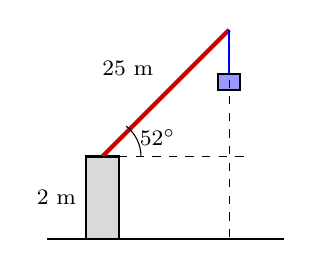
\begin{tikzpicture}[scale=0.7]
  % Mặt đất
  \draw[thick] (-0.5,0) -- (3.8,0);
  % Tháp cẩu
  \draw[thick, fill=gray!30] (0.2,0) rectangle (0.8,1.5);
  \node[left] at (0.2,0.75) {\footnotesize $2\text{ m}$};
  % Cánh tay đòn
  \draw[line width=1.5pt, red!80!black] (0.5,1.5) -- (2.8,3.8);
  \node[above left] at (1.6,2.8) {\footnotesize $25\text{ m}$};
  % Đường nằm ngang gióng góc
  \draw[dashed] (0.5,1.5) -- (3.2,1.5);
  % Góc nâng 52 độ
  \draw (0.5,1.5) ++(0:0.7) arc (0:52:0.7);
  \node at (1.5,1.85) {\footnotesize $52^\circ$};
  % Dây móc hàng
  \draw[thick, blue] (2.8,3.8) -- (2.8,3.0);
  \draw[thick, fill=blue!40] (2.6,2.7) rectangle (3.0,3.0);
  \draw[dashed] (2.8,3.8) -- (2.8,0);
\end{tikzpicture}
\end{minipage}

\vspace{1.5mm}
\textbf{Câu 18.} Một hình quạt tròn có bán kính $R = 15\text{ cm}$ và góc ở tâm tương ứng là $72^\circ$. Tính diện tích của hình quạt tròn đó theo $\pi$ và làm tròn đến hàng phần mười (lấy $\pi \approx 3{,}14$, đơn vị: $\text{cm}^2$).

\vspace{4mm}
\noindent
\textbf{\large II. TỰ LUẬN (3,0 điểm).} \textit{Thí sinh trình bày lời giải chi tiết vào tờ giấy thi.}

\vspace{2mm}
\textbf{Câu 19 (1,0 điểm).}
\begin{itemize}
  \item[a)] \textit{(0,5 điểm)} Giải hệ phương trình: $\begin{cases} 2x + 5y = 11 \\ 3x - 2y = 7 \end{cases}$.
  \item[b)] \textit{(0,5 điểm)} Cho biểu thức $P = \left( \dfrac{1}{\sqrt{x}-1} + \dfrac{1}{\sqrt{x}+1} \right) : \dfrac{2\sqrt{x}}{x-1}$ với $x > 0, x \ne 1$. Rút gọn biểu thức $P$.
\end{itemize}

\vspace{2mm}
\textbf{Câu 20 (1,5 điểm).} Cho đường tròn $(O; R)$, từ một điểm $M$ nằm ngoài đường tròn kẻ hai tiếp tuyến $MA, MB$ với $(O)$ ($A$ và $B$ là hai tiếp điểm). Kẻ cát tuyến $MCD$ không đi qua tâm $O$ ($C$ nằm giữa $M$ và $D$). Gọi $H$ là giao điểm của đoạn thẳng $MO$ và dây cung $AB$.
\begin{itemize}
  \item[a)] \textit{(0,75 điểm)} Chứng minh rằng đường thẳng $MO$ vuông góc với dây cung $AB$ tại $H$ và $MA^2 = MH \cdot MO$.
  \item[b)] \textit{(0,75 điểm)} Chứng minh rằng $MC \cdot MD = MH \cdot MO$, từ đó suy ra bốn điểm $C, H, O, D$ cùng thuộc một đường tròn.
\end{itemize}

\vspace{2mm}
\textbf{Câu 21 (0,5 điểm).}
\begin{itemize}
  \item[a)] \textit{(0,25 điểm)} Bác Hai có một mảnh vườn hình chữ nhật có diện tích $S = 200\text{ m}^2$. Bác dự định làm hàng rào bao quanh ba phía của mảnh vườn (gồm hai chiều rộng và một chiều dài), phía chiều dài còn lại giáp với bờ tường hoa kiên cố của nhà văn hóa thôn nên không cần rào. Hỏi các kích thước (chiều dài và chiều rộng) của mảnh vườn phải bằng bao nhiêu mét để tổng chiều dài hàng rào cần làm là ngắn nhất?
  \item[b)] \textit{(0,25 điểm)} Cho ba số thực dương $a, b, c$ thỏa mãn điều kiện $ab + bc + ca = 3$. Tìm giá trị nhỏ nhất của biểu thức:
  \[
  Q = \dfrac{a^2}{b+c} + \dfrac{b^2}{c+a} + \dfrac{c^2}{a+b}.
  \]
\end{itemize}

\vspace{4mm}
\begin{center}
\textbf{---------- HẾT ----------}\\
\textit{(Cán bộ coi thi không giải thích gì thêm)}
\end{center}

\end{document}
